\documentclass{article}
\usepackage[utf8]{inputenc}
\usepackage{graphicx}
\usepackage{float}
\usepackage{amsmath}
\usepackage[title]{appendix}
\usepackage{subcaption}
\usepackage[usenames,dvipsnames]{color}
\usepackage[hyphen]{url}
\def\UrlBreaks{\do\/\do-}
\usepackage{hyperref}
\setlength{\tabcolsep}{5pt}
\usepackage{multirow}
\usepackage{comment}
\usepackage{stackengine}

\usepackage{natbib}
\bibliographystyle{abbrvnat}
\setcitestyle{authoryear,open={(},close={)}}
\usepackage{aas_macros}


\usepackage{indentfirst}
\usepackage[width=1.15\textwidth,aboveskip=2pt]{caption}
\graphicspath{ {./Images/} }
\usepackage{comment}
\usepackage[a4paper,width=165mm,top=25.4mm,bottom=25.4mm]{geometry}

\title{Silicon Potential Energy Coefficients \\ Artificial Neural Network Framework}
\author{Lauren Higgins \\ Univeristy of Missouri - Kansas City}
\date{July 26 2022}

\begin{document}

\maketitle
\begin{abstract}
    Deriving potential equations for amorphous solids is important, but computationally 
    expensive. One potential way to decrease computational cost is to train machine learning 
    networks to predict potential equations. Using \citep{Yanxon2020} force field neural 
    network (NN) as a template, I wrote similar NN that would instead predict 
    potential energy function coefficients. Due to time constraints, the input bispectrum 
    coefficients were not ready to train the NN. Instead, I focused on three main areas (i) 
    code that will effectively load data files of different configurations, (ii) potential data
    pre-processing methods, (iii) and the few lines of code that house the neural network. The 
    framework will be tested in the future.
\end{abstract}

\section{Introduction}

Computing potential energy (PE) coefficients is computationally expensive. Historically, the 
quantum mechanic time dependent description of large systems of atoms have been described using
molecular dynamics and ab initio molecular dynamics. 
Methodologies to make the process run faster often include machine learning techniques 
\citep{Yanxon2020}. This work uses \textit{ab initio} calculation of PE coefficients from the 
orthogonalized linear combination of atomic orbitals (OLCAO) method as the output pair to the 
input bispectrum coefficients to train a machine learning neural network (NN) that will predict
the PE coefficients and decrease computation cost by orders of magnitude \cite{Yanxon2020}.   

In more detail, this paper is outlined as follows. Section 2 gives context to why modeling 
potential functions at the surface of materials is computationally difficult and, if utilized 
well, can be made less expensive with the use of machine learning techniques. A full 
description of \cite{Yanxon2020} NN and how the approach given in this paper compares to it is 
contained in Section 3. Due 
to time constraints, I was unable to obtain the input bispectrum coefficients to train the 
network, so Section 4 outlines how I commented the code and wrote a \texttt{.readme} 
for future students to easily understand both the framework I designed and the structure of the
output data. I also discuss future work to both better understanding what parts of the 
potential function are most important and to optimize the input data and NN.

\section{Background}

Described in this section is the atomic physics theory that defines the structure of solids and
how neural networks can aid in predicting the time dependent behavior of large groups of atoms.

\subsection{Atomistic Modeling}

A commonly used method to calculate the potential equations for amorphous solids is the 
orthogonalized linear combination of atomic orbitals (OLCAO) method \citep{Rulis}. The 
functional form of the electron repulsion and exchange-correlation portion of the potential energy
equation is shown in equation \ref{pot}.
\begin{align}
    V(r) & = \Sigma V(r)_{i} && \nonumber\\
         & = \Sigma A_{j} e^{\alpha_{j}r^{2}}
    \label{pot}
\end{align}

\noindent
where the first summation is over potential sites (also coincident with atomic sites) and
where A and $\alpha$ are the characteristic coefficients of the potential function at each site "i". 
The coefficient, A, changes with each term and type but $\alpha$ is static across all 
variations of the types of atoms of a given element in the configuration. Using OLCAO to compute 
the coefficients in equation \ref{pot} is very computationally expensive. One way to decrease the 
computational expense is to create machine learning algorithms to predict the coefficents A$_j{}$ in 
V(r) without a lengthy iterative (self-consistent field) process. 

%Add bispectrum coefficients. Use equation 4, Yanxon et al. 2020

\subsection{Neural Network Machine Learning}

Using neural networks to predict potential energy equations can decrease the computational 
cost by 2 to 4 orders of magnitudes \cite{Yanxon2020}. However, training the NN does require the 
use of \textit{ab initio} calculations from the OLCAO method. Once the applicable network is trained, 
it is designed to be applied to new scenarios independent of the previously more  
computationally expensive methods. In other words, the intent is for the NN to be trained using a 
set of smaller and simpler systems and then applied to larger and more complex systems. Networks 
can have varying levels of complexity, but they generally follow the schematic shown in Figure 
\ref{NN_sch} with an input layer, weights to 
each of the inputs that create hidden layer(s). Then, weights to the hidden layers, that create
the output layer. In our case, the input layer are the bispectrum coefficients for a given model
and the output layer is the PE coefficients for the same site. The weights are scalars that define 
how important each input value is for the NN. The hidden layer is predicted based on the weights. 
The specifics of both the weights and hidden layers are discussed further in Section 3.2.

\begin{figure}[H]
    \centering
    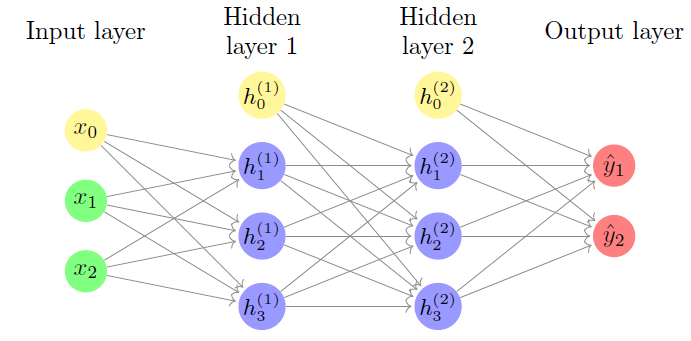
\includegraphics[scale=1.6]{Images/NN_size.png}
    \caption{Shown here is a generic neural network (NN) framework schematic. Reading it from left to right, this figure shows the input layer (yellow and green circles) connected to the first set of weights (black lines). Then, two sets of hidden layers (yellow and purple circles) connected by weights (black lines). Last, the output layer (red circles), connected to the second hidden layer via weights (black lines). \citep{NN}}
    \label{NN_sch}
\end{figure}

\section{Methods}

I designed a neural network that was modeled off of \cite{Yanxon2020} where my 
input/output pairs are the bispectrum coefficients and potential energy function coefficients 
for a given atom of silicon. For supervised training purposes, the output values were generated 
using the minimum basis functions needed to calculate the 
potential energy coefficients A and $\alpha$. This section will outline the data used to train 
the NN and the NN framework created to predict the potential energy coefficient, A. The output 
data was created in time to test the NN, but the input data was not, instead I focused on 
devising several ways to pre-process the input data, better read in the data files, and using 
\cite{Yanxon2020} as a template for the NN.

\subsection{Preparing the Data}

Bispectrum coefficients are the input data used that describe the local environment of an atom 
in some atomic scale system. They are the expansion coefficients of 4D hyperspherical harmonics 
and follow Equation \ref{bi_eq} \citep{Yanxon2020}. 

\begin{equation}
    B_{i}^{l_{1}, l_{2}, l} = \sum_{m, m'=-l}^{l} (c^{l}_{m',m})^{*} \sum_{m_{1}, m'_{1}=-l_{1}}^{l_{1}} \sum_{m_{2}, m'_{2}=-l_{2}}^{l_{2}}
    \times \; c^{l_{1}}_{m'_{1},m_{1}} c^{l_{2}}_{m'_{2},m_{2}} H^{l,m,m'}_{l_{1},m_{1},m'_{1},l_{2},m_{2},m'_{2}}
    \label{bi_eq}
\end{equation}
\noindent
where $H^{l,m,m'}_{l_{1},m_{1},m'_{1},l_{2},m_{2},m'_{2}}$ acts like Clebsch-Gordan coefficients on a 3-sphere 
\citep{Yanxon2020}. The bispectrum coefficients needed for this work are still in preperation and will be used
once they are generated. The remaining work on training data was centered around the output potential energy 
coefficients.

In this case, the atomic structure for different silicon materials 
was used to provide a diverse set of environments. The output training data are the potential 
function coefficients for each atom. This data came from a set of Si systems (amorphous silicon 
with various scales of bond length, a silicon self-interstitial model, a silicon passive defect 
model, and perfect crystalline silicon) with varied configuration characteristics in terms 
of bond angles, bond lengths, and impurities in the substrate. Our output data pair was calculated 
using the minimum basis functions needed to calculate the potential energy coefficients A and $\alpha$. 

I considered several ways to pre-process the data for effective use in the neural netowrk. 
Normalizing (or min-max scaling) the data is a key step for machine learning. Without 
normalization, data categories that are scaled differently 
will confuse the network. Scikit \texttt{Normalization()} uses gradient descent to 
independently normalize the input data samples by rescaling all samples with at least one 
non-zero component. I also wrote code for data visualization 
to find any necessary trends in distribution to optimize data stratification, if needed. 
(This code can be found in the repository hosted by Professor Rulis' research group.) This step 
is necessary in machine learning when there is a known distribution of the data that, without 
considering this distribution, would greatly negatively bias the output. 

\subsection{Neural Network Framework}

Along with numpy, I utilized Scikit packages to create the neural network (NN) framework. The 
specific package for the NN pipeline that mimics \cite{Yanxon2020} is the \texttt{MLPRegressor()}.
\texttt{MLPRegressor()} is a multi-layer perceptron classifier that optimizes the log-loss 
function using either limited-memory Broyden-Fletcher-Goldfarb-Shanno (LBFGS) or stochastic gradient descent. 
The parameters of \texttt{MLPRegressor()} can
be carefully selected to recreate schematic shown in Figure \ref{Yan_sche}. I chose to use ADAM; 
the same algorithm used in \cite{Yanxon2020}. It is a stochastic gradient-based optimizer that was
developed by \cite{Adam}.Theirs is likely more robust; however, for the purposes of this project 
my version was close enough to create comparable results that can be augmented for robustness in 
the future.

\begin{figure}
    \centering
    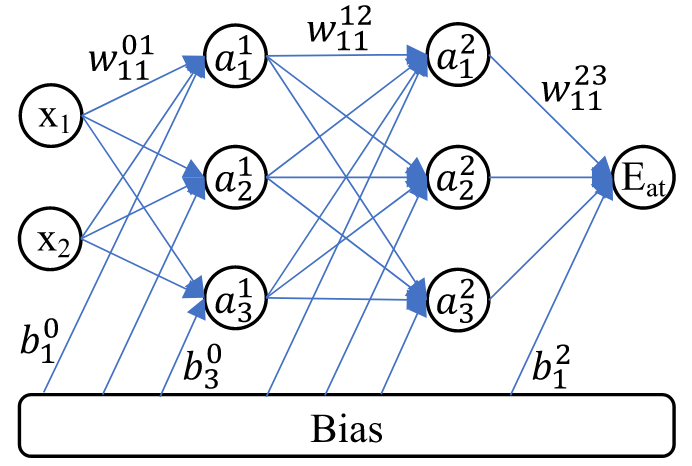
\includegraphics[scale=0.7]{Images/Yan_sche.png}
    \caption{This image is the schematic of the Neural Network from \cite{Yanxon2020}. Here the x 
    layer is the input layer, the two a layers are the hidden layers, and E$_{at}$ is the energy 
    output layer. The blue lines between input, hidden, and output layers show the weights, 
    w$^{ij}_{11}$. The blue lines from the Bias to each layer after the input layer, b, represent 
    the bias factored into each layer.}
    \label{Yan_sche}
\end{figure}

\section{Future Work}

It is a generalized way to read in data files whose structure are 
dependent on the structure file.

Due to time constraints, the bispectrum coefficients were not generated in time to train the 
NN. Instead, I heavily commented my code and created a \texttt{.readme} for the next student 
who wants to utilize this method to train a NN to predict potential energy coefficients. I 
also added in notes about writing a generalized way to read in data files whose structure are 
dependent on the structure file. Correctly dealing with the variety of complications that can 
arise will require more sophisticaed data parsing and may lead to multiple ANNs. Some example 
complications include: the need to deal with more than one element in a given model (which 
affects the potential coefficient data file *and* the construction of the bispectrum coefficients); 
the possibliity that one potential *type* might be applied to more than one atomic *site*; and that 
an ANN for Si in one set of systems may not be easily applicable to Si in other systems (i.e., 
there may be limits on the usefulness of including so many different environments for training). 

In terms of the NN framework, future work includes using the NN I wrote and training it using the 
input/out pairs of bispectrum coefficients to potential energy coefficients, A. Questions to 
explore could be:

\begin{enumerate}
    \item Does the sign and magnitude of the respective A make that term more important than others?
    \item How sensitive is V(r) to small changes in the A's?
\end{enumerate}
\noindent
Answers to the aforementioned questions could lead to important data pre-processing methods, 
threshold values for ADAM, or any key parameter within the NN framework. 

\clearpage
%References
\bibliography{citations}

\end{document}
